\section{Illustration: a pre-registered replication of Clark and Ravazzolo (2015)}\label{sec:replication}\label{sec:cr}
% -----------------------------------------------------------------------------------------------
% Drafting notes (not typeset).
%
% Number discipline (OUTLINE.md §11):
%   * every number of the acceptance run is an \acc{} placeholder, filled from
%     benchmarks/reports/clark_ravazzolo_acceptance.json (main repo; to be committed, TODO 2);
%   * numbers of the first full run (report benchmarks/reports/clark_ravazzolo.json, committed in
%     551f181, code 4bb978a, path-conditioned LPD) are history and are wrapped in \fullrun{};
%   * numbers of the fit-level convergence diagnostic and of the estimator review are quoted from
%     the committed pre-registration (c823d20) and tagged [PREREG];
%   * every LPD number names the estimator that produced it.
%
% Placeholder grammar used in \acc{...} (mirrors the report dict built in main() and the
% helpers relative_table(), verdicts(), criteria() and ordering_stage() of
% benchmarks/clark_ravazzolo.py at c823d20):
%   a.b.c        object keys;
%   ['k']        a key with characters outside [A-Za-z0-9_] (model names such as 'SV(rw)',
%                'AR-SV(0.9)') and every horizon key: horizon keys are the strings '1','2','4','8';
%   [f=v,g=w]    the element(s) of a list whose fields match (string values in single quotes,
%                booleans as true/false), e.g. verdicts.full[model='SV(rw)',horizon=1,convergence_gate=true];
%                criteria[id=4] is the criterion with "id": 4;
%   [*]          every element of a list or every value of an object;
%   min(P), max(P)       over the values selected by P;
%   count(P = v)         the number of values selected by P that equal v;
%   absent(k)            true when the top-level key k is not in the JSON.
% Shares (converged.*, converged_sv, converged_constant) are fractions in [0, 1].
% -----------------------------------------------------------------------------------------------
\newsavebox{\crheadlinebox}% holds the tabular of the headline table (tab:cr-headline)

\subsection{Role and target}\label{sec:replication-role}\label{sec:replication-target}

The replication is one of the project's Phase~2 exit criteria, and it is qualitative: the target
is the ranking reported by \citet{clark2015macroeconomic}, that VARs with stochastic volatility
beat homoskedastic VARs in density forecasts, not their numbers cell by cell. % [R] SPEC.md §10.7 l.552; DESIGN exit-criteria map (WP23)
It exercises the whole stack on real data: a pinned, checksummed download, the composition API,
the look-ahead-free backtest, the scores, \code{compare()} with its convergence gate, and
\code{ordering_sensitivity}. It illustrates the workflow; it does not test the econometric claim
beyond these data and these models.

We compare with the numbers of the working paper, \citet[Tables~1--3, United States, VAR
block]{clark2012macroeconomic}, which the script hard-codes for display; the tables of the
published article were not accessed. % [R] benchmarks/clark_ravazzolo.py CR_FULL l.147, CR_PRE_DLPS l.167 (c823d20); N08 §C1, §C5
\todo{TODO 22: obtain the JAE tables and re-check, or keep this sentence; resolve N08's ``every
number re-read'' (40) against the 56 numbers quoted.}
Their VAR(4) has a Minnesota prior without cross-variable shrinkage (tightness $0.2$, $1/l^2$ lag
decay, zero prior means) and a normal-diffuse error covariance \citep{kadiyala1997numerical}. Their
VAR-SV has random-walk log-volatilities, sampled with the single-move step of
\citet{jacquier1994bayesian}; the variants we use are AR-SV with a nearly fixed autoregressive
coefficient and SV with Student-$t$ errors with fixed degrees of freedom $d$
\citep{jacquier2004bayesian}. % [R] N08 §C3
They do not state the recursive ordering, so we run all $24$ orderings, with the table order GDP,
INFL, UR, TBILL as the identity ordering. % [R] N08 §C2, §D item 2

\subsection{Data and models}\label{sec:replication-data}\label{sec:replication-models}

FRED-QD and FRED-MD, vintage 2026-09 \citep{mccracken2021fredqd,mccracken2016fredmd}, are
downloaded on demand and checked against their SHA-256 checksums. GDP growth and inflation are
$100\,\Delta\log$ of \code{GDPC1} and \code{GDPCTPI} as non-annualised quarterly rates (FRED-QD has
no GDP deflator); \code{UNRATE} and \code{TB3MS} enter in levels. Estimation starts in 1965Q1, as in
\citet{clark2011realtime}, because FRED-QD starts in 1959. % [R] N08 §C2 (1965Q1 precedent; CR start 1955Q1)
The forecasts are pseudo real time on the
final vintage, not on real-time vintages \citep{croushore2001realtime}. \cref{tab:TabF2} lists the
series and transformations, and \cref{app:cr} every deviation from the original design. % [V] benchmarks/clark_ravazzolo.py load_data l.236, DEVIATIONS l.1380
Two properties are asserted at run time. The quarterly \code{UNRATE} and \code{TB3MS} of FRED-QD
must be within-quarter means of the monthly FRED-MD values (to $0.01$); the largest difference was
\fullrun{$3.3\times10^{-5}$} in the first full run % [FULL: data_checks.aggregation.*.max_abs_diff]
and is \acc{data_checks.aggregation.UNRATE.max_abs_diff} and
\acc{data_checks.aggregation.TB3MS.max_abs_diff} in the acceptance run. And there is no
look-ahead: at 1985Q1, 2007Q4 and 2011Q2 the resolved prior, its hyperparameters and the padded
data are bitwise identical when the vintage itself is cut at the origin
(\acc{data_checks.in_window.identical}). This check runs for the primary arm only.
% [V] benchmarks/clark_ravazzolo.py assert_quarterly_averages l.269, assert_in_window l.296, called in main() l.1496 with mods[PRIMARY_SV]

Every arm shares the mean block
\code{Linear(prior=Minnesota(form='reduced', hierarchy='fixed', lambda_=0.2, alpha=2, cross=1, mean=0))},
$p = 4$: Clark and Ravazzolo's prior on the reduced form, sampled with the corrected triangular
algorithm \citep{carriero2022corrigendum}. % [V] benchmarks/clark_ravazzolo.py minnesota l.325
The volatility arms (\cref{tab:TabF3}) are: % [V] benchmarks/clark_ravazzolo.py models l.330, structural_models l.345
the baseline \code{Constant('iw_equivalent')}, the prior of \citet{chan2022asymmetric} under which
$\Sigma$ is inverse-Wishart and the reduced form is order invariant, in place of the normal-diffuse
VAR; the primary arm SV(rw), Clark and Ravazzolo's VAR-SV; the library's AR(1) default SV;
SV(rw,t10), with $\nu$ fixed at their $d = 10$, so that, by construction, the library's
grid-bound warning on $\nu$ fires at every origin; AR-SV(0.9), whose $(\phi + 1)/2 \sim
\mathrm{Beta}(71.25, 3.75)$ matches the mean and standard deviation of their $a_1 \sim N(0.9,
0.05^2)$; and a structural Mode~I pair, \code{Constant('ig')} against SV(rw), as a robustness
check. Apart from the $\nu$ prior of SV(rw,t10) and the $\phi$ prior of AR-SV(0.9), the SV priors
are the library defaults (\cref{sec:framework:vol}). Clark and Ravazzolo's
$\mathrm{IG}(1/2, 0.0175)$ prior on the random-walk innovation variance is not adopted, and no prior
was tuned. % [V] DEVIATIONS item 5; docstring l.66-67

\subsection{Evaluation design}\label{sec:replication-design}

Forecasts come from an expanding window at the $106$ origins 1985Q1--2011Q2, of which the $92$ up
to 2007Q4 form the pre-crisis sample, for $h = 1, 2, 4, 8$ quarters ahead. Each origin is a
separate MCMC fit with its own fit seed. % [V] benchmarks/clark_ravazzolo.py FULL, PRE_CRISIS_END, HORIZONS l.141-143
Under an expanding window the Diebold--Mariano test with the Harvey--Leybourne--Newbold correction
\citep{diebold1995comparing,harvey1997testing} is not formally valid
\citep{clark2001tests,giacomini2006tests}, so its $p$-values are descriptive, and a ``better''
verdict can only come through the model confidence set \citep[MCS;][]{hansen2011model}.

The primary score is the Rao--Blackwellised (RB) log predictive density of
\cref{sec:eval-lpd}: path-conditioned at $h > 1$ in the first full run, path-integrated in
the acceptance run; the two coincide at $h = 1$. The acceptance run also reports the
path-conditioned score on the same draws, as a secondary number that never enters a rule.
% [V] benchmarks/clark_ravazzolo.py relative_table l.479 (dlps_conditioned, dlpd_conditioned); LPD_INTEGRATED_DEVIATION l.1372
For parity we report Clark and Ravazzolo's Gaussian-approximation score
\citep{adolfson2007forecasting}, computed from the same draws' mean and covariance. It is
$-\tfrac12$ times the Dawid--Sebastiani score up to a constant \citep{dawid1999coherent}, proper but
not strictly proper \citep{gneiting2007strictly,kruger2021predictive}, and we flag the cells in
which its sign differs from that of the RB score. CRPS and RMSE ratios complete the set.
$\Delta$LPS is the mean per-origin log-score difference against \code{Constant}, in nats per
quarter. Verdicts are reported with the convergence gate on, as \code{compare()} returns them, and
off.

An origin is \emph{RB-degenerate} at horizon $h$ when the delta-method MCSE of the joint RB score of
either arm is at least $0.9$: the weights then sit on about one draw, and the MCSE saturates near
one nat however far off the estimate is. % [R] benchmarks/clark_ravazzolo.py RB_CEILING docstring l.355-359
\todo{TODO 14: cite the MCSE weight bound of \cref{app:mcse-bound} here only after it is
derived and unit-tested.}
The flag is descriptive: flagged origins are kept, because dropping exactly the tail origins would
bias the comparison. The ordering stage runs \code{ordering_sensitivity(mode='backtest',
design='all')} with one noise replicate for SV(rw) and \code{Constant}, then a \code{compare()}
verdict per ordering, each ordering with its own backtest seed. % [V] benchmarks/clark_ravazzolo.py ordering_stage l.840; src/rai_bvar/structural/ordering.py docstring l.1137-1151
\code{Constant('iw_equivalent')} is order invariant, so its spread across orderings is Monte Carlo
noise, which makes it a negative control.

\subsection{Criteria}\label{sec:replication-criteria}

The replication plan states six criteria in words, and the script turns them into rules; both are
in \cref{tab:cr-criteria}, the rules verbatim. The operationalisations are the project's own:
``about 1'' became $\leq 1.02$, and ``systematically'' became at least $3$ of $4$ joint horizons or
$8$ of $16$ marginal cells. Criterion~4's rule compares $h = 8$ with $h = 1$ only, whereas the
wording says the gain ``shrinks or turns negative''; the rule was not changed after the first run.
Only criterion~6 uses the convergence gate, and it uses $h = 1$ scores only, which do not depend on
the estimator. % [V] benchmarks/clark_ravazzolo.py criteria l.666-834; N08 §C5

\begin{table}[tbp]
\centering
\small
\caption{The six acceptance criteria: the qualitative wording of the replication plan, the rule as
coded (verbatim from \code{criteria()}), and the outcome in the first full run (report at 551f181,
path-conditioned LPD, $4 \times 5000$ draws) and in the pre-registered acceptance run
(path-integrated LPD, $4 \times 20{,}000$ draws). The first-run column is history.}
\label{tab:cr-criteria}\label{Tab12}\label{tab:Tab12}
% data: acceptance JSON criteria[*].{id,met,rule,detail}; first run benchmarks/reports/clark_ravazzolo.json criteria (551f181); script tab_cr_criteria.py (OUTLINE §14)
\begin{tabular}{@{}p{0.02\textwidth}p{0.23\textwidth}p{0.39\textwidth}p{0.08\textwidth}p{0.16\textwidth}@{}}
\toprule
\# & Wording (plan) & Rule as coded & First run & Acceptance \\
\midrule
1 & SV beats Constant in average LPD at $h = 1, 2$ for all four variables in both samples; the joint
  $h = 1$ gain is clearly positive
  & $\Delta$LPS(SV(rw) $-$ Constant) $> 0$ at $h = 1, 2$ for all four variables in the full and
  pre-crisis samples, and the joint $\Delta$LPD at $h = 1$ $> 0$ with one-sided DM/HLN $p < 0.10$
  in both samples
  & \fullrun{met} & \acc{criteria[id=1].met} \\
2 & CRPS ratio $< 1$ at $h \leq 2$ for all four variables
  & CRPS ratio SV(rw)/Constant $< 1$ at $h = 1, 2$ for all four variables (full sample)
  & \fullrun{met} & \acc{criteria[id=2].met} \\
3 & RMSE ratios $\leq$ about 1 at short horizons
  & RMSE ratio SV(rw)/Constant $\leq 1.02$ (`about 1') at $h = 1, 2$ for all four variables (full
  sample); CR's gains for GDP and the bill are 5--10\%
  & \fullrun{met} & \acc{criteria[id=3].met} \\
4 & Full sample: the $h = 8$ gain shrinks or turns negative for UR and the bill; pre-crisis it stays
  positive for GDP and inflation
  & full sample: $\Delta$LPS($h$=8) $<$ $\Delta$LPS($h$=1) for UR and TBILL; pre-crisis:
  $\Delta$LPS($h$=8) $> 0$ for GDP and INFL
  & \fullrun{not met} & \acc{criteria[id=4].met} \\
5 & Neither SV-$t$ nor AR-SV systematically beats RW or AR SV
  & neither SV(rw,t10) nor AR-SV(0.9) is better than both SV(rw) and SV (one-sided DM/HLN
  $p < 0.10$, positive $\Delta$LPD) at $\geq 3$ of 4 joint horizons or $\geq 8$ of 16 marginal
  cells (full sample)
  & \fullrun{met} & \acc{criteria[id=5].met} \\
6 & \code{compare()} says ``better'' (DM one-sided at 10\% for at least GDP and the bill at
  $h = 1$) in all 24 orderings, or the report states which fail
  & in every one of the 24 orderings: \code{compare()} verdict SV(rw) vs Constant at $h = 1$ is
  `better', and the one-sided DM/HLN $p$-value of the marginal log score is $< 0.10$ for GDP and
  TBILL at $h = 1$
  & \fullrun{not met} & \acc{criteria[id=6].met} \\
\bottomrule
\end{tabular}
\end{table}
% [FULL: criteria[*].met] first-run column; [V] rule strings identical in benchmarks/clark_ravazzolo.json (551f181) and the code at c823d20

\subsection{The first full run (history)}\label{sec:replication-first-run}

The numbers of this subsection are history, not results. The first full run used $4 \times 5000$
kept draws (burn-in $1000$), $1000$ forecast draws and the path-conditioned LPD; an earlier attempt
had aborted on the float64 failure of \cref{sec:robustness-f2} (run history in
\cref{tab:TabF1}). It met criteria \fullrun{1, 2, 3 and 5} and missed \fullrun{4 and 6}.
% [FULL: config; criteria[*].met] benchmarks/reports/clark_ravazzolo.json (551f181, code 4bb978a); [R] issue #3 04:10Z

Criterion~4 failed on one cell. In the full sample the unemployment gain at $h = 8$,
\fullrun{$+1.954$}, exceeded the one at $h = 1$, \fullrun{$+0.159$}. At three 2007--08 origins the
per-origin difference was \fullrun{$+41.6$}, \fullrun{$+41.4$} and \fullrun{$+40.4$} nats, the median difference was
\fullrun{$+0.099$}, and \fullrun{12} origins were RB-degenerate at $h = 8$; the Gaussian
approximation gave \fullrun{$-0.499$}. Across arms and samples the RB and Gaussian $\Delta$LPS
differed in sign in \fullrun{28} marginal and \fullrun{8} joint cells, all at $h \geq 2$.
% [FULL: criteria[id=4].detail; relative.full['SV(rw)'].variables.UR['8'].{dlps,dlps_median,dlps_top,rb_degenerate,dlps_gauss}; rb_gauss_disagree counts recomputed]

Criterion~6 failed on the convergence gate alone. SV(rw) was ``better'' at $h = 1$ in \fullrun{0}
of $24$ orderings with the gate on and in \fullrun{24} of $24$ with it off. It converged at
\fullrun{57--82\%} of origins across orderings (\code{Constant}: \fullrun{100\%}). In the report's
example warning for each SV arm (main stage), a fit missed on one $\sigma$ quantity out of 13
primary quantities (random-walk arms) or 21 (AR arms), with $\hat R$ \fullrun{1.012--1.020} and bulk
ESS \fullrun{537--743}. With the gate off, all four SV arms were ``better'' than \code{Constant} at
$h = 1$ in the full sample through the MCS route (total $\Delta$LPD \fullrun{$+85.7$ to $+87.5$}
nats, MCSEs \fullrun{1.00--1.06}). % [FULL: criteria[id=6].detail; orderings.per_ordering[*].converged_*; warnings[arm]['MCMC not converged'].example (SV(rw) 1 of 13, R-hat 1.015, ESS 618; SV 1 of 21, 1.013, 550; SV(rw,t10) 1 of 13, 1.020, 537; AR-SV(0.9) 1 of 21, 1.012, 743); verdicts.full (gate off, h=1: MCS25 model in, reference out)]
Inflation gains were \fullrun{1.6 to 3.2} times Clark and Ravazzolo's (our RB score against their
Gaussian one); final-vintage \code{GDPCTPI} and the \code{iw_equivalent} baseline are candidate
causes that we did not test. % [FULL: relative.full['SV(rw)'].variables.INFL[*].dlps vs CR_FULL]

\subsection{Diagnosis and the pre-registration}\label{sec:replication-prereg}

\paragraph{(a) The budget.}
SV(rw) was refitted at the main-stage fit seeds under several MCMC budgets, with fit-level
diagnostics only and no forecasts or scores. In the identity ordering $72$ of $106$ origins
converged at $4 \times 5000$, $79$ with a burn-in of $5000$, $92$ with $8$ chains, and $106$ at
$4 \times 20{,}000$ (largest $\hat R$ $1.0061$, smallest bulk ESS $1763$); in the two worst
orderings the counts went from $71$ and $63$ to $106$. All $520 + 424$ fits finished without error,
and every fit that failed at the base budget failed on a $\sigma$ quantity with $\hat R < 1.03$,
which the pre-registration reads as $\hat R$ sampling noise at a bulk ESS near $600$.
% [PREREG] benchmarks/reports/clark_ravazzolo_preregistration.md item 1 (c823d20). Per-fit records in docs/paper/figures/data/convergence_diagnostic/{identity_ordering,worst_orderings}.jsonl + conv_diag.py (paper worktree, untracked); recounted from them: 72/79/92/106; 71,63 -> 106,106; max R-hat 1.0061/1.0049/1.0046; min ESS 1763/1689/1717; every failing base fit has a sigma quantity among its failures. Stays [PREREG] until committed.
\todo{TODO 4: commit the diagnostic script and output to the main repository (source of
\cref{tab:TabF6}).}
The first run holds a seed-to-seed check: its main stage and ordering~0 of its ordering stage fit
the same models in the same ordering under different seeds, and SV(rw) converged at \fullrun{72}
against \fullrun{69} origins (joint $h = 1$ $\Delta$LPD \fullrun{$+0.809$} against
\fullrun{$+0.838$}). % [FULL: converged.full['SV(rw)']; orderings.per_ordering[ordering=0].{converged_sv,dlpd_h1}]
Near the threshold the converged count moves with the seed, so budgets are best sized with fit-only
diagnostics before any score exists.

\paragraph{(b) The estimator.}
The criterion-4 cell was driven by the tail failure of the path-conditioned estimator
(\cref{sec:eval-tail}, \cref{fig:lpd-estimators}); the acceptance run uses the path-integrated
estimator. % [PREREG] "Why there is a second run"; [R] NOTES 8b (review of the quick run); [FULL: 12 RB-degenerate origins at UR h=8]

\paragraph{(c) Forecast draws.}
The path-integrated estimator is still an average over draws, and at crisis origins its weights
concentrate. In the review of the estimator at the acceptance MCMC budget
(\cref{sec:eval-tail}), Constant's estimate at 2008Q2, unemployment $h = 8$, had a standard
deviation of $0.75$--$1.06$ nats across thinning offsets with $1000$ forecast draws and $0.09$--$0.19$
with $8000$; the MCMC error across fit seeds, about $1.3$ nats, does not shrink with more forecast
draws.
% [PREREG] item 3; [R] NOTES 8b addendum (main repo, b9c66c0)

\paragraph{What was registered.}
The pre-registration, committed in c823d20, changes exactly three settings: $4 \times 20{,}000$
kept draws (burn-in $1000$) for every MCMC arm in every stage, the path-integrated LPD as the
primary score, and $8000$ forecast draws per origin. Data, models, priors, origins, horizons, seeds,
the ordering stage, the coded criteria, the $95\%$ gate and the descriptive RB-degenerate flag are
unchanged. % [PREREG] "What changes", "What does not change"; [V] benchmarks/clark_ravazzolo.py CONFIGS l.186-199
It is explicit about its limits: ``These changes are motivated by that failure analysis, so the
run is not blind to the previous results. What is pre-registered is that the settings below were
fixed before any score of the new run existed, and that the criteria are evaluated on them as
coded, whatever the outcome.'' It states in advance that criterion~4 may still fail on
unemployment (in the review of the quick run, the estimate with corrected tail origins was about
$+0.23$ at $h = 8$ against $+0.157$ at $h = 1$), that criterion~6 is expected to pass if the gate is
met, and that no further run with other settings is made after the scores are seen, except to fix
a bug.
% [PREREG] "Stated in advance"; the review numbers are of the quick run: benchmarks/clark_ravazzolo.py RELIABILITY_NOTE l.953 (dossier 06 §7.6 fact-check)

\paragraph{Provenance.}
The run was launched from a detached worktree at c823d20 with a clean tree, and therefore after the
pre-registration had been committed.
% [R] OUTLINE §0.4 (commit 2026-10-23 12:10:45 EDT; launch 12:10 EDT, same minute: the order rests on the worktree being at c823d20, to be confirmed by versions.git_commit and the archived log)
\todo{TODO 2: commit the acceptance JSON and report; archive the run log with its UTC start time.}
The report labels itself the acceptance run only when the registered settings were used, every
stage ran and the tracked files were unchanged (\code{acceptance_gaps()}); the fields that decide
this are listed in \cref{app:cr}. Here the configuration is \acc{config.name}, the commit
\acc{versions.git_commit}, and modified tracked files \acc{versions.git_dirty}.
% Appendix F lists: config.lpd_method, config.draws, config.mcmc.{chains,draws,burn}, config.seed, absent(pending)
% [V] benchmarks/clark_ravazzolo.py acceptance_gaps l.1022, is_acceptance l.1058; tests/unit/test_clark_ravazzolo_script.py::test_acceptance_label_needs_the_registered_run

\subsection{Results of the acceptance run}\label{sec:replication-results}

\paragraph{Reading rules.}
Which numbers may move between the two runs was written down before the acceptance numbers
existed. % [R] docs/paper/dossiers/06_empirical.md §9.5, OUTLINE §11.9 (paper worktree, untracked; no acceptance JSON existed then, OUTLINE §0.4)
\todo{Commit these reading rules before the acceptance JSON is committed, so that their timing is
checkable, or drop the clause ``before the acceptance numbers existed''.}
\begin{itemize}
  \item[A.] \emph{Estimator:} every RB $\Delta$LPS and $\Delta$LPD at $h \geq 2$, the DM $p$-values
    at $h \geq 2$, the RB/Gaussian sign disagreements, the criterion-4 cells, the variant
    comparisons and the ordering spread at $h \geq 2$.
  \item[B.] \emph{Monte Carlo noise only:} all $h = 1$ LPD numbers, CRPS and RMSE ratios, Gaussian
    scores and $h = 1$ DM $p$-values; between the quick ($4 \times 2000$) and the first full run,
    the full-sample $h = 1$ $\Delta$LPS of SV(rw) moved by at most \fullrun{$0.003$} per marginal
    cell (\fullrun{$0.002$} joint), and over all arms and both samples by at most \fullrun{$0.0044$}
    per marginal cell (\fullrun{$0.0122$} joint).
    % [FULL]/[R] computed from clark_ravazzolo_quick.json and clark_ravazzolo.json (relative[sample][arm], h=1): SV(rw) full max 0.0027 marginal, 0.0019 joint; all arms and samples max 0.0044 marginal (pre_crisis SV(rw)), 0.0122 joint (full AR-SV(0.9)). The quick report predates f60d736 (OUTLINE risk 19): context only.
  \item[C.] \emph{Budget:} converged shares, gate-on verdicts, criterion~6's gate-on count, the MC
    standard errors of the totals and the run time.
  \item[D.] \emph{Unchanged by design:} data checks, models, priors, origins, rules and fit seeds.
\end{itemize}

\paragraph{Criteria and headline.}
\cref{tab:cr-criteria} gives each criterion's outcome; the details of criteria 4 and 6, including
the secondary numbers that do not enter the rules, are \acc{criteria[id=4].detail} and
\acc{criteria[id=6].detail}. \cref{tab:cr-headline} is the headline comparison. The joint $h = 1$
gain is \acc{relative.full['SV(rw)'].joint['1'].dlpd} nats per quarter (descriptive one-sided DM
$p$ \acc{relative.full['SV(rw)'].joint['1'].dm_p_better}). The unemployment cell at $h = 8$ is
\acc{relative.full['SV(rw)'].variables.UR['8'].dlps} path-integrated,
\acc{relative.full['SV(rw)'].variables.UR['8'].dlps_conditioned} path-conditioned and
\acc{relative.full['SV(rw)'].variables.UR['8'].dlps_gauss} under the Gaussian approximation, with
\acc{relative.full['SV(rw)'].joint['8'].rb_degenerate} RB-degenerate origins. Across arms and
samples the RB and Gaussian $\Delta$LPS differ in sign in
\acc{count(relative[*][*].variables[*][*].rb_gauss_disagree = true)} marginal and
\acc{count(relative[*][*].joint[*].rb_gauss_disagree = true)} joint cells.

\begin{table}[tbp]
\centering
\footnotesize
\setlength{\tabcolsep}{3pt}
\caption{SV(rw) against \code{Constant}, full sample (106 origins), acceptance run.
$\Delta$LPS: mean per-origin log-score difference in nats per quarter, path-integrated RB
estimator (primary), path-conditioned RB estimator on the same draws (secondary, never in a rule)
and Gaussian approximation (parity metric). ``Sign'': RB and Gaussian $\Delta$LPS differ in sign.
``Degen.'': RB-degenerate origins (joint MCSE $\geq 0.9$ for either arm; the count is per horizon
and the same for all variables). DM $p$: one-sided DM/HLN $p$-value for ``SV(rw) is better'',
descriptive under the expanding window. CR: Clark and Ravazzolo's VAR-SV against VAR, working-paper
Tables 1--3, Gaussian-approximation log score.}
\label{tab:cr-headline}\label{Tab13}\label{tab:Tab13}
% The tabular is boxed and shrunk to \textwidth only if it is wider (the long \acc placeholders of the draft); filled with numbers it keeps its natural size.
% data: acceptance JSON relative.full['SV(rw)'].variables[v][h].{dlps,dlps_conditioned,dlps_gauss,rb_gauss_disagree,rb_degenerate,dm_p_better,crps_ratio,rmse_ratio}, .joint[h].{dlpd,dlpd_conditioned,dlpd_gauss,rb_gauss_disagree,rb_degenerate,dm_p_better}; CR columns [R] benchmarks/clark_ravazzolo.py CR_FULL l.147 (= clark2012macroeconomic Tables 1-3); script tab_cr_headline.py (OUTLINE §14)
\sbox{\crheadlinebox}{%
\begin{tabular}{@{}llrrrcrrrrrrr@{}}
\toprule
 & & \multicolumn{3}{c}{$\Delta$LPS} & & & & \multicolumn{2}{c}{Ratio} & \multicolumn{3}{c}{CR} \\
\cmidrule(lr){3-5}\cmidrule(lr){9-10}\cmidrule(l){11-13}
Var. & $h$ & Integr. & Cond. & Gauss. & Sign & Degen. & DM $p$ & CRPS & RMSE & $\Delta$LPS & CRPS & RMSE \\
\midrule
GDP & 1 & \acc{relative.full['SV(rw)'].variables.GDP['1'].dlps} & \acc{relative.full['SV(rw)'].variables.GDP['1'].dlps_conditioned} & \acc{relative.full['SV(rw)'].variables.GDP['1'].dlps_gauss} & \acc{relative.full['SV(rw)'].variables.GDP['1'].rb_gauss_disagree} & \acc{relative.full['SV(rw)'].variables.GDP['1'].rb_degenerate} & \acc{relative.full['SV(rw)'].variables.GDP['1'].dm_p_better} & \acc{relative.full['SV(rw)'].variables.GDP['1'].crps_ratio} & \acc{relative.full['SV(rw)'].variables.GDP['1'].rmse_ratio} & $+0.193$ & 0.864 & 0.896 \\
 & 2 & \acc{relative.full['SV(rw)'].variables.GDP['2'].dlps} & \acc{relative.full['SV(rw)'].variables.GDP['2'].dlps_conditioned} & \acc{relative.full['SV(rw)'].variables.GDP['2'].dlps_gauss} & \acc{relative.full['SV(rw)'].variables.GDP['2'].rb_gauss_disagree} & \acc{relative.full['SV(rw)'].variables.GDP['2'].rb_degenerate} & \acc{relative.full['SV(rw)'].variables.GDP['2'].dm_p_better} & \acc{relative.full['SV(rw)'].variables.GDP['2'].crps_ratio} & \acc{relative.full['SV(rw)'].variables.GDP['2'].rmse_ratio} & $+0.133$ & 0.856 & 0.878 \\
 & 4 & \acc{relative.full['SV(rw)'].variables.GDP['4'].dlps} & \acc{relative.full['SV(rw)'].variables.GDP['4'].dlps_conditioned} & \acc{relative.full['SV(rw)'].variables.GDP['4'].dlps_gauss} & \acc{relative.full['SV(rw)'].variables.GDP['4'].rb_gauss_disagree} & \acc{relative.full['SV(rw)'].variables.GDP['4'].rb_degenerate} & \acc{relative.full['SV(rw)'].variables.GDP['4'].dm_p_better} & \acc{relative.full['SV(rw)'].variables.GDP['4'].crps_ratio} & \acc{relative.full['SV(rw)'].variables.GDP['4'].rmse_ratio} & $+0.090$ & 0.890 & 0.932 \\
 & 8 & \acc{relative.full['SV(rw)'].variables.GDP['8'].dlps} & \acc{relative.full['SV(rw)'].variables.GDP['8'].dlps_conditioned} & \acc{relative.full['SV(rw)'].variables.GDP['8'].dlps_gauss} & \acc{relative.full['SV(rw)'].variables.GDP['8'].rb_gauss_disagree} & \acc{relative.full['SV(rw)'].variables.GDP['8'].rb_degenerate} & \acc{relative.full['SV(rw)'].variables.GDP['8'].dm_p_better} & \acc{relative.full['SV(rw)'].variables.GDP['8'].crps_ratio} & \acc{relative.full['SV(rw)'].variables.GDP['8'].rmse_ratio} & $+0.060$ & 0.927 & 1.007 \\
\addlinespace
INFL & 1 & \acc{relative.full['SV(rw)'].variables.INFL['1'].dlps} & \acc{relative.full['SV(rw)'].variables.INFL['1'].dlps_conditioned} & \acc{relative.full['SV(rw)'].variables.INFL['1'].dlps_gauss} & \acc{relative.full['SV(rw)'].variables.INFL['1'].rb_gauss_disagree} & \acc{relative.full['SV(rw)'].variables.INFL['1'].rb_degenerate} & \acc{relative.full['SV(rw)'].variables.INFL['1'].dm_p_better} & \acc{relative.full['SV(rw)'].variables.INFL['1'].crps_ratio} & \acc{relative.full['SV(rw)'].variables.INFL['1'].rmse_ratio} & $+0.075$ & 0.954 & 0.966 \\
 & 2 & \acc{relative.full['SV(rw)'].variables.INFL['2'].dlps} & \acc{relative.full['SV(rw)'].variables.INFL['2'].dlps_conditioned} & \acc{relative.full['SV(rw)'].variables.INFL['2'].dlps_gauss} & \acc{relative.full['SV(rw)'].variables.INFL['2'].rb_gauss_disagree} & \acc{relative.full['SV(rw)'].variables.INFL['2'].rb_degenerate} & \acc{relative.full['SV(rw)'].variables.INFL['2'].dm_p_better} & \acc{relative.full['SV(rw)'].variables.INFL['2'].crps_ratio} & \acc{relative.full['SV(rw)'].variables.INFL['2'].rmse_ratio} & $+0.083$ & 0.944 & 0.949 \\
 & 4 & \acc{relative.full['SV(rw)'].variables.INFL['4'].dlps} & \acc{relative.full['SV(rw)'].variables.INFL['4'].dlps_conditioned} & \acc{relative.full['SV(rw)'].variables.INFL['4'].dlps_gauss} & \acc{relative.full['SV(rw)'].variables.INFL['4'].rb_gauss_disagree} & \acc{relative.full['SV(rw)'].variables.INFL['4'].rb_degenerate} & \acc{relative.full['SV(rw)'].variables.INFL['4'].dm_p_better} & \acc{relative.full['SV(rw)'].variables.INFL['4'].crps_ratio} & \acc{relative.full['SV(rw)'].variables.INFL['4'].rmse_ratio} & $+0.155$ & 0.895 & 0.915 \\
 & 8 & \acc{relative.full['SV(rw)'].variables.INFL['8'].dlps} & \acc{relative.full['SV(rw)'].variables.INFL['8'].dlps_conditioned} & \acc{relative.full['SV(rw)'].variables.INFL['8'].dlps_gauss} & \acc{relative.full['SV(rw)'].variables.INFL['8'].rb_gauss_disagree} & \acc{relative.full['SV(rw)'].variables.INFL['8'].rb_degenerate} & \acc{relative.full['SV(rw)'].variables.INFL['8'].dm_p_better} & \acc{relative.full['SV(rw)'].variables.INFL['8'].crps_ratio} & \acc{relative.full['SV(rw)'].variables.INFL['8'].rmse_ratio} & $+0.138$ & 0.887 & 0.883 \\
\addlinespace
UR & 1 & \acc{relative.full['SV(rw)'].variables.UR['1'].dlps} & \acc{relative.full['SV(rw)'].variables.UR['1'].dlps_conditioned} & \acc{relative.full['SV(rw)'].variables.UR['1'].dlps_gauss} & \acc{relative.full['SV(rw)'].variables.UR['1'].rb_gauss_disagree} & \acc{relative.full['SV(rw)'].variables.UR['1'].rb_degenerate} & \acc{relative.full['SV(rw)'].variables.UR['1'].dm_p_better} & \acc{relative.full['SV(rw)'].variables.UR['1'].crps_ratio} & \acc{relative.full['SV(rw)'].variables.UR['1'].rmse_ratio} & $+0.162$ & 0.922 & 0.967 \\
 & 2 & \acc{relative.full['SV(rw)'].variables.UR['2'].dlps} & \acc{relative.full['SV(rw)'].variables.UR['2'].dlps_conditioned} & \acc{relative.full['SV(rw)'].variables.UR['2'].dlps_gauss} & \acc{relative.full['SV(rw)'].variables.UR['2'].rb_gauss_disagree} & \acc{relative.full['SV(rw)'].variables.UR['2'].rb_degenerate} & \acc{relative.full['SV(rw)'].variables.UR['2'].dm_p_better} & \acc{relative.full['SV(rw)'].variables.UR['2'].crps_ratio} & \acc{relative.full['SV(rw)'].variables.UR['2'].rmse_ratio} & $+0.098$ & 0.897 & 0.930 \\
 & 4 & \acc{relative.full['SV(rw)'].variables.UR['4'].dlps} & \acc{relative.full['SV(rw)'].variables.UR['4'].dlps_conditioned} & \acc{relative.full['SV(rw)'].variables.UR['4'].dlps_gauss} & \acc{relative.full['SV(rw)'].variables.UR['4'].rb_gauss_disagree} & \acc{relative.full['SV(rw)'].variables.UR['4'].rb_degenerate} & \acc{relative.full['SV(rw)'].variables.UR['4'].dm_p_better} & \acc{relative.full['SV(rw)'].variables.UR['4'].crps_ratio} & \acc{relative.full['SV(rw)'].variables.UR['4'].rmse_ratio} & $-0.182$ & 0.906 & 0.914 \\
 & 8 & \acc{relative.full['SV(rw)'].variables.UR['8'].dlps} & \acc{relative.full['SV(rw)'].variables.UR['8'].dlps_conditioned} & \acc{relative.full['SV(rw)'].variables.UR['8'].dlps_gauss} & \acc{relative.full['SV(rw)'].variables.UR['8'].rb_gauss_disagree} & \acc{relative.full['SV(rw)'].variables.UR['8'].rb_degenerate} & \acc{relative.full['SV(rw)'].variables.UR['8'].dm_p_better} & \acc{relative.full['SV(rw)'].variables.UR['8'].crps_ratio} & \acc{relative.full['SV(rw)'].variables.UR['8'].rmse_ratio} & $-0.707$ & 1.001 & 0.971 \\
\addlinespace
TBILL & 1 & \acc{relative.full['SV(rw)'].variables.TBILL['1'].dlps} & \acc{relative.full['SV(rw)'].variables.TBILL['1'].dlps_conditioned} & \acc{relative.full['SV(rw)'].variables.TBILL['1'].dlps_gauss} & \acc{relative.full['SV(rw)'].variables.TBILL['1'].rb_gauss_disagree} & \acc{relative.full['SV(rw)'].variables.TBILL['1'].rb_degenerate} & \acc{relative.full['SV(rw)'].variables.TBILL['1'].dm_p_better} & \acc{relative.full['SV(rw)'].variables.TBILL['1'].crps_ratio} & \acc{relative.full['SV(rw)'].variables.TBILL['1'].rmse_ratio} & $+0.284$ & 0.822 & 0.933 \\
 & 2 & \acc{relative.full['SV(rw)'].variables.TBILL['2'].dlps} & \acc{relative.full['SV(rw)'].variables.TBILL['2'].dlps_conditioned} & \acc{relative.full['SV(rw)'].variables.TBILL['2'].dlps_gauss} & \acc{relative.full['SV(rw)'].variables.TBILL['2'].rb_gauss_disagree} & \acc{relative.full['SV(rw)'].variables.TBILL['2'].rb_degenerate} & \acc{relative.full['SV(rw)'].variables.TBILL['2'].dm_p_better} & \acc{relative.full['SV(rw)'].variables.TBILL['2'].crps_ratio} & \acc{relative.full['SV(rw)'].variables.TBILL['2'].rmse_ratio} & $+0.043$ & 0.915 & 0.944 \\
 & 4 & \acc{relative.full['SV(rw)'].variables.TBILL['4'].dlps} & \acc{relative.full['SV(rw)'].variables.TBILL['4'].dlps_conditioned} & \acc{relative.full['SV(rw)'].variables.TBILL['4'].dlps_gauss} & \acc{relative.full['SV(rw)'].variables.TBILL['4'].rb_gauss_disagree} & \acc{relative.full['SV(rw)'].variables.TBILL['4'].rb_degenerate} & \acc{relative.full['SV(rw)'].variables.TBILL['4'].dm_p_better} & \acc{relative.full['SV(rw)'].variables.TBILL['4'].crps_ratio} & \acc{relative.full['SV(rw)'].variables.TBILL['4'].rmse_ratio} & $-0.304$ & 1.010 & 0.974 \\
 & 8 & \acc{relative.full['SV(rw)'].variables.TBILL['8'].dlps} & \acc{relative.full['SV(rw)'].variables.TBILL['8'].dlps_conditioned} & \acc{relative.full['SV(rw)'].variables.TBILL['8'].dlps_gauss} & \acc{relative.full['SV(rw)'].variables.TBILL['8'].rb_gauss_disagree} & \acc{relative.full['SV(rw)'].variables.TBILL['8'].rb_degenerate} & \acc{relative.full['SV(rw)'].variables.TBILL['8'].dm_p_better} & \acc{relative.full['SV(rw)'].variables.TBILL['8'].crps_ratio} & \acc{relative.full['SV(rw)'].variables.TBILL['8'].rmse_ratio} & $-0.403$ & 1.059 & 0.990 \\
\addlinespace
joint & 1 & \acc{relative.full['SV(rw)'].joint['1'].dlpd} & \acc{relative.full['SV(rw)'].joint['1'].dlpd_conditioned} & \acc{relative.full['SV(rw)'].joint['1'].dlpd_gauss} & \acc{relative.full['SV(rw)'].joint['1'].rb_gauss_disagree} & \acc{relative.full['SV(rw)'].joint['1'].rb_degenerate} & \acc{relative.full['SV(rw)'].joint['1'].dm_p_better} &  &  &  &  &  \\
 & 2 & \acc{relative.full['SV(rw)'].joint['2'].dlpd} & \acc{relative.full['SV(rw)'].joint['2'].dlpd_conditioned} & \acc{relative.full['SV(rw)'].joint['2'].dlpd_gauss} & \acc{relative.full['SV(rw)'].joint['2'].rb_gauss_disagree} & \acc{relative.full['SV(rw)'].joint['2'].rb_degenerate} & \acc{relative.full['SV(rw)'].joint['2'].dm_p_better} &  &  &  &  &  \\
 & 4 & \acc{relative.full['SV(rw)'].joint['4'].dlpd} & \acc{relative.full['SV(rw)'].joint['4'].dlpd_conditioned} & \acc{relative.full['SV(rw)'].joint['4'].dlpd_gauss} & \acc{relative.full['SV(rw)'].joint['4'].rb_gauss_disagree} & \acc{relative.full['SV(rw)'].joint['4'].rb_degenerate} & \acc{relative.full['SV(rw)'].joint['4'].dm_p_better} &  &  &  &  &  \\
 & 8 & \acc{relative.full['SV(rw)'].joint['8'].dlpd} & \acc{relative.full['SV(rw)'].joint['8'].dlpd_conditioned} & \acc{relative.full['SV(rw)'].joint['8'].dlpd_gauss} & \acc{relative.full['SV(rw)'].joint['8'].rb_gauss_disagree} & \acc{relative.full['SV(rw)'].joint['8'].rb_degenerate} & \acc{relative.full['SV(rw)'].joint['8'].dm_p_better} &  &  &  &  &  \\
\bottomrule
\end{tabular}}%
\ifdim\wd\crheadlinebox>\textwidth
  \resizebox{\textwidth}{!}{\usebox{\crheadlinebox}}%
\else
  \usebox{\crheadlinebox}%
\fi
\end{table}

\paragraph{Pre-crisis sample and the other arms.}
Criterion~4 also needs the pre-crisis gains of GDP and inflation at $h = 8$ to stay positive
(\cref{tab:TabF4}). The GDP cell was \fullrun{$+0.108$} (path-conditioned) and
\fullrun{$-0.004$} (Gaussian) in the first run % [FULL: relative.pre_crisis['SV(rw)'].variables.GDP['8'].{dlps,dlps_gauss}]
and is \acc{relative.pre_crisis['SV(rw)'].variables.GDP['8'].dlps} (path-integrated),
\acc{relative.pre_crisis['SV(rw)'].variables.GDP['8'].dlps_conditioned} (path-conditioned) and
\acc{relative.pre_crisis['SV(rw)'].variables.GDP['8'].dlps_gauss} (Gaussian) here; inflation is
\acc{relative.pre_crisis['SV(rw)'].variables.INFL['8'].dlps}. The budget diagnostic covered SV(rw)
only, in three orderings at the main-stage seeds, so the other SV arms may still miss the gate and
stay ``inconclusive'' (\cref{tab:TabF5}). Over the full sample the converged shares are
\acc{converged.full['SV(rw)']} for SV(rw), \acc{converged.full.SV} for SV,
\acc{converged.full['SV(rw,t10)']} for SV(rw,t10), \acc{converged.full['AR-SV(0.9)']} for
AR-SV(0.9) and \acc{converged.full.Constant} for \code{Constant}. At $h = 1$ the SV(rw) verdict is
\acc{verdicts.full[model='SV(rw)',horizon=1,convergence_gate=true].verdict} with the gate on and
\acc{verdicts.full[model='SV(rw)',horizon=1,convergence_gate=false].verdict} with it off.
\todo{After the JSON is in: state the route of every ``better'' verdict from
\code{verdicts.full[*].reasons} and \code{model_in_mcs}/\code{reference_in_mcs}; under the
expanding window it can only be the MCS.}

\paragraph{Ordering robustness.}
\cref{fig:cr-orderings} shows the $h = 1$ gain in each of the $24$ orderings. In the first run the
joint $h = 1$ range across orderings was \fullrun{$0.083$} nats against a gain of
\fullrun{$0.809$}, and the per-variable gains were \fullrun{2.2--7.8} times their ranges.
% [FULL: orderings.results['SV(rw)'].joint_lpd_range['1'], .summary[horizon=1].lpd_range; relative.full['SV(rw)'].variables[*]['1'].dlps]
In the acceptance run the joint $h = 1$ range is
\acc{orderings.results['SV(rw)'].joint_lpd_range['1']} nats, the joint gain runs from
\acc{min(orderings.per_ordering[*].dlpd_h1)} to \acc{max(orderings.per_ordering[*].dlpd_h1)}, SV(rw)
converged at \acc{min(orderings.per_ordering[*].converged_sv)} to
\acc{max(orderings.per_ordering[*].converged_sv)} of origins, and the verdict is ``better'' in
\acc{count(orderings.per_ordering[*].verdict_h1 = 'better')} of $24$ orderings with the gate on and
\acc{count(orderings.per_ordering[*].verdict_h1_ungated = 'better')} with it off. In the first run
the order-invariant \code{Constant} arm was flagged ``material'' at joint $h = 2$ and unemployment
$h = 8$, both path-conditioned cells with a one-replicate noise floor.
% [FULL: orderings.results.Constant.material = true; summary rows (joint,2) lpd_range 0.189, SNR 14.3; (UR,8) 1.233, SNR 7.5]
Here the flag is \acc{orderings.results.Constant.material}
(\acc{orderings.results.Constant.summary[material=true]}); because the arm is order invariant in
theory, we read a flag on it as a limitation of the noise floor (\cref{sec:limitations}),
not as evidence of order dependence.
\cref{fig:FigF2} compares the converged shares per ordering of the two runs.
\todo{TODO 5: add the per-origin export (\code{docs/paper/data/cr_acceptance_per_origin.csv}) for
\cref{fig:FigF1,fig:FigF3}, or drop both figures.}

\begin{figure}[tbp]
\centering
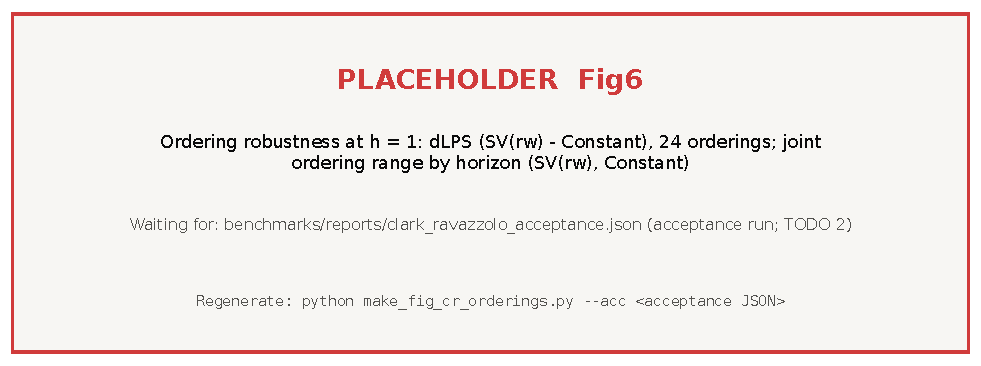
\includegraphics[width=\textwidth]{figures/fig_cr_orderings.pdf}
\caption{Ordering robustness, acceptance run. Left: $\Delta$LPS (SV(rw) $-$ \code{Constant}) at
$h = 1$ per variable and joint, one point per ordering (24), with the identity ordering marked; each
column gives the spread across orderings and SV(rw)'s signal-to-noise ratio, the quantity the
materiality flag compares with 3. Right: joint ordering range by horizon for SV(rw) and for the
order-invariant \code{Constant} arm (negative control), with flagged cells marked. At $h \geq 2$
the scores are path-integrated.}
\label{fig:cr-orderings}\label{Fig6}\label{fig:Fig6}
% data: acceptance JSON orderings.per_ordering[*].{ordering,label,dlps_h1,dlpd_h1}, orderings.results[*].summary[*].{variable,horizon,lpd_range,lpd_range_snr,material}; script figures/make_fig_cr_orderings.py (sigma_MC is not in the report, so no noise band is drawn)
\end{figure}

\paragraph{Interpretation.}
The pre-registration fixed how a failure of criterion~4 is reported: as a difference from Clark
and Ravazzolo, attributed with evidence where there is any to the final-vintage data, the
\code{iw_equivalent} baseline or the default SV priors, with no setting tuned in response.
% [PREREG] "Stated in advance"
Reading rule~B is the check on the $h = 1$ numbers: they should differ from the first run's by
Monte Carlo noise only. The run-level warnings (\acc{warnings}) are listed in
\cref{app:cr}.
\todo{After the acceptance JSON is committed: two or three sentences of interpretation from the
numbers above, within these branches only.}

\subsection{Caveats}\label{sec:replication-caveats}

The illustration is limited by the following: final-vintage instead of real-time data; the working
paper's numbers instead of the article's; Chan's \code{iw_equivalent} baseline instead of the
normal-diffuse VAR, and the library's SV priors instead of Clark and Ravazzolo's; descriptive
significance, with verdicts that come through the MCS, whose validity in this setting is open;
operational thresholds of our own choosing;
a pre-registration that is not blind; one backtest seed in the main stage; and a change of the
primary estimator between the runs at $h > 1$, which is why every LPD number above names its
estimator. Finally, the primary arm, reduced form $\times$ SV(rw), and its $t$ variant are validated
only through their parts: at the commit of the run they have no registered Geweke or SBC row and
no contract-test fit (\cref{sec:validation-coverage}). % [V] at c823d20 (= HEAD d58c9ef for code): src/rai_bvar/validation/joint.py _COMPOSITIONS (RW only in row 14, structural_sv_rw); tests/mcmc/forecast/mcmc_fits.py COMPOSITIONS (12, none reduced SV(rw), none reduced SV(rw,t))
\todo{TODO 3: row~18, \code{reduced_sv_rw} (reduced form $\times$ SV(rw)), and a \code{reduced-SV(rw)} contract fit were committed in 7f410dc, after the acceptance commit c823d20; the SV(rw, $t$) variant is still not covered (SBC needs a per-row $t_{\max}$ of 400). The caveat stays true of the run's commit; once the release records exist, add that the arm has since been validated as a row of its own, here and in \cref{sec:validation-coverage,sec:limitations}.}
